%%%%%%
% $Beschreibung: Frontblende $
% $Autor: ter Veen $
% $Datum: 15.06.2024 $
% $Version: 1 $
% $Pfad: SchrittmotorArduino/Manual/Tikz/Frontblende.tex $
%
%%%%%%

	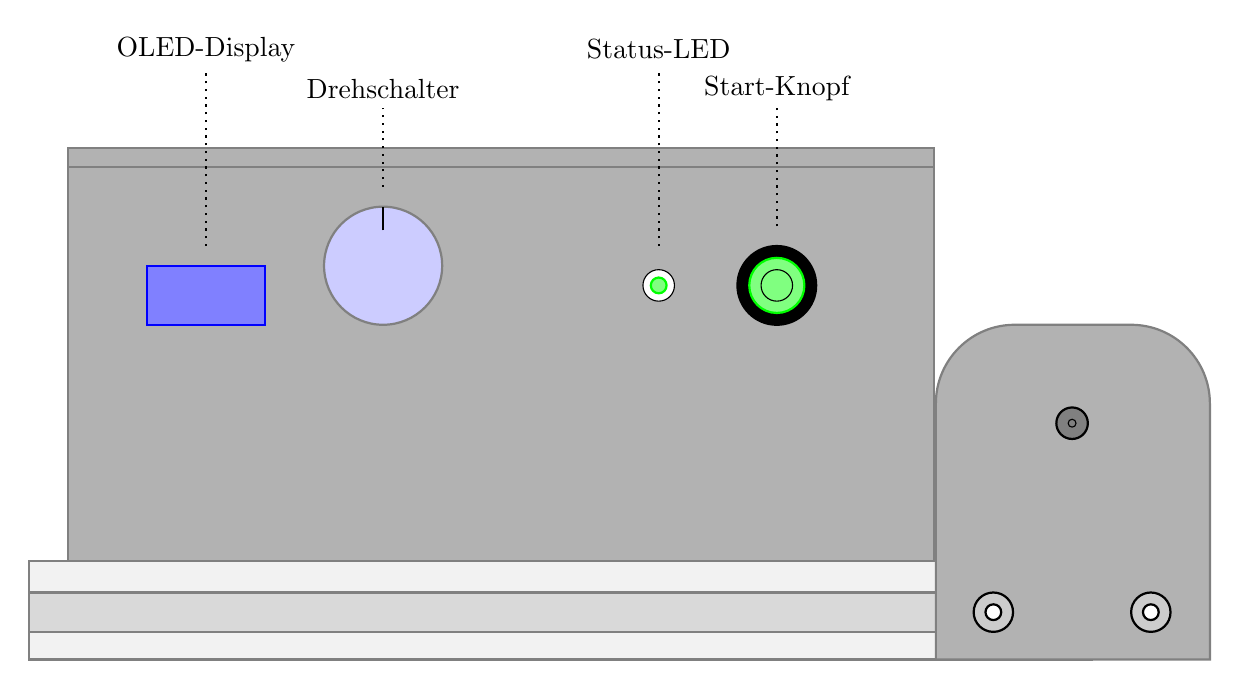
\begin{tikzpicture}
		%Gehäusedeckel
		\draw[gray, thick, fill=gray!60] (2,8) rectangle (13,8.25);
		
		% Gehäuse
		\draw[gray, thick, fill=gray!60] (2,3) rectangle (13,8);
		
		% Alu-Profil
		\draw[gray, thick, fill=gray!10] (1.5,1.75) rectangle (15,3);
		\draw[gray, thick, fill=gray!30] (1.5,2.1) rectangle (15,2.6);
		
		 % Halterung
		\draw[gray, thick, fill=gray!60] 
		(13.02,1.75) -- (13.02,5) arc[start angle=180, end angle=90, radius=1cm] -- (15.5,6) arc[start angle=90, end angle=0, radius=1cm] -- (16.5,1.75) -- 
		cycle;
		% Lagerung Zahnrad
		\draw[black, thick, fill=gray] (14.75,4.75) circle (0.2);
		\draw[black, thin, fill=gray] (14.75,4.75) circle (0.05);
		%Befestigungsschrauben
		\draw[black, thick, fill=gray!40] (13.75,2.35) circle (0.25);
		\draw[black, thick, fill=white] (13.75,2.35) circle (0.1);
		\draw[black, thick, fill=gray!40] (15.75,2.35) circle (0.25);
		\draw[black, thick, fill=white] (15.75,2.35) circle (0.1);

	
		% Draw the OLED-Display
		\draw[blue, thick, fill=blue!50] (3,6) rectangle (4.5,6.75);

		% Draw the Drehschalter (Knob)
		\draw[gray, thick, fill=blue!20] (6,6.75) circle (0.75);
		\draw[thick] (6,7.2) -- (6,7.5);
		
		% Draw the Status-LED
		\draw[black, thin, fill=white] (9.5,6.5) circle (0.2);
		\draw[green, thick, fill=green!50] (9.5,6.5) circle (0.1);
		
		% Draw the Start-Knopf (Button)
		\draw[black, thick, fill=black] (11,6.5) circle (0.5);
		\draw[green, thick, fill=green!50] (11,6.5) circle (0.35);
		\draw[black] (11,6.5) circle (0.2);
		
		% Dotted lines for labels
		\draw[dotted, thick] (3.75,7) -- (3.75,9.25);
		\draw[dotted, thick] (6,7.75) -- (6,8.75);
		\draw[dotted, thick] (9.5,7) -- (9.5,9.25);
		\draw[dotted, thick] (11,7.25) -- (11,8.75);
		
		% Labels
		\node[] at (3.75,9.5) {OLED-Display};
		\node[] at (6,9) {Drehschalter};
		\node[] at (9.5,9.5) {Status-LED};
		\node[] at (11,9) {Start-Knopf};
	\end{tikzpicture}
